\begin{figure}
\begin{center}
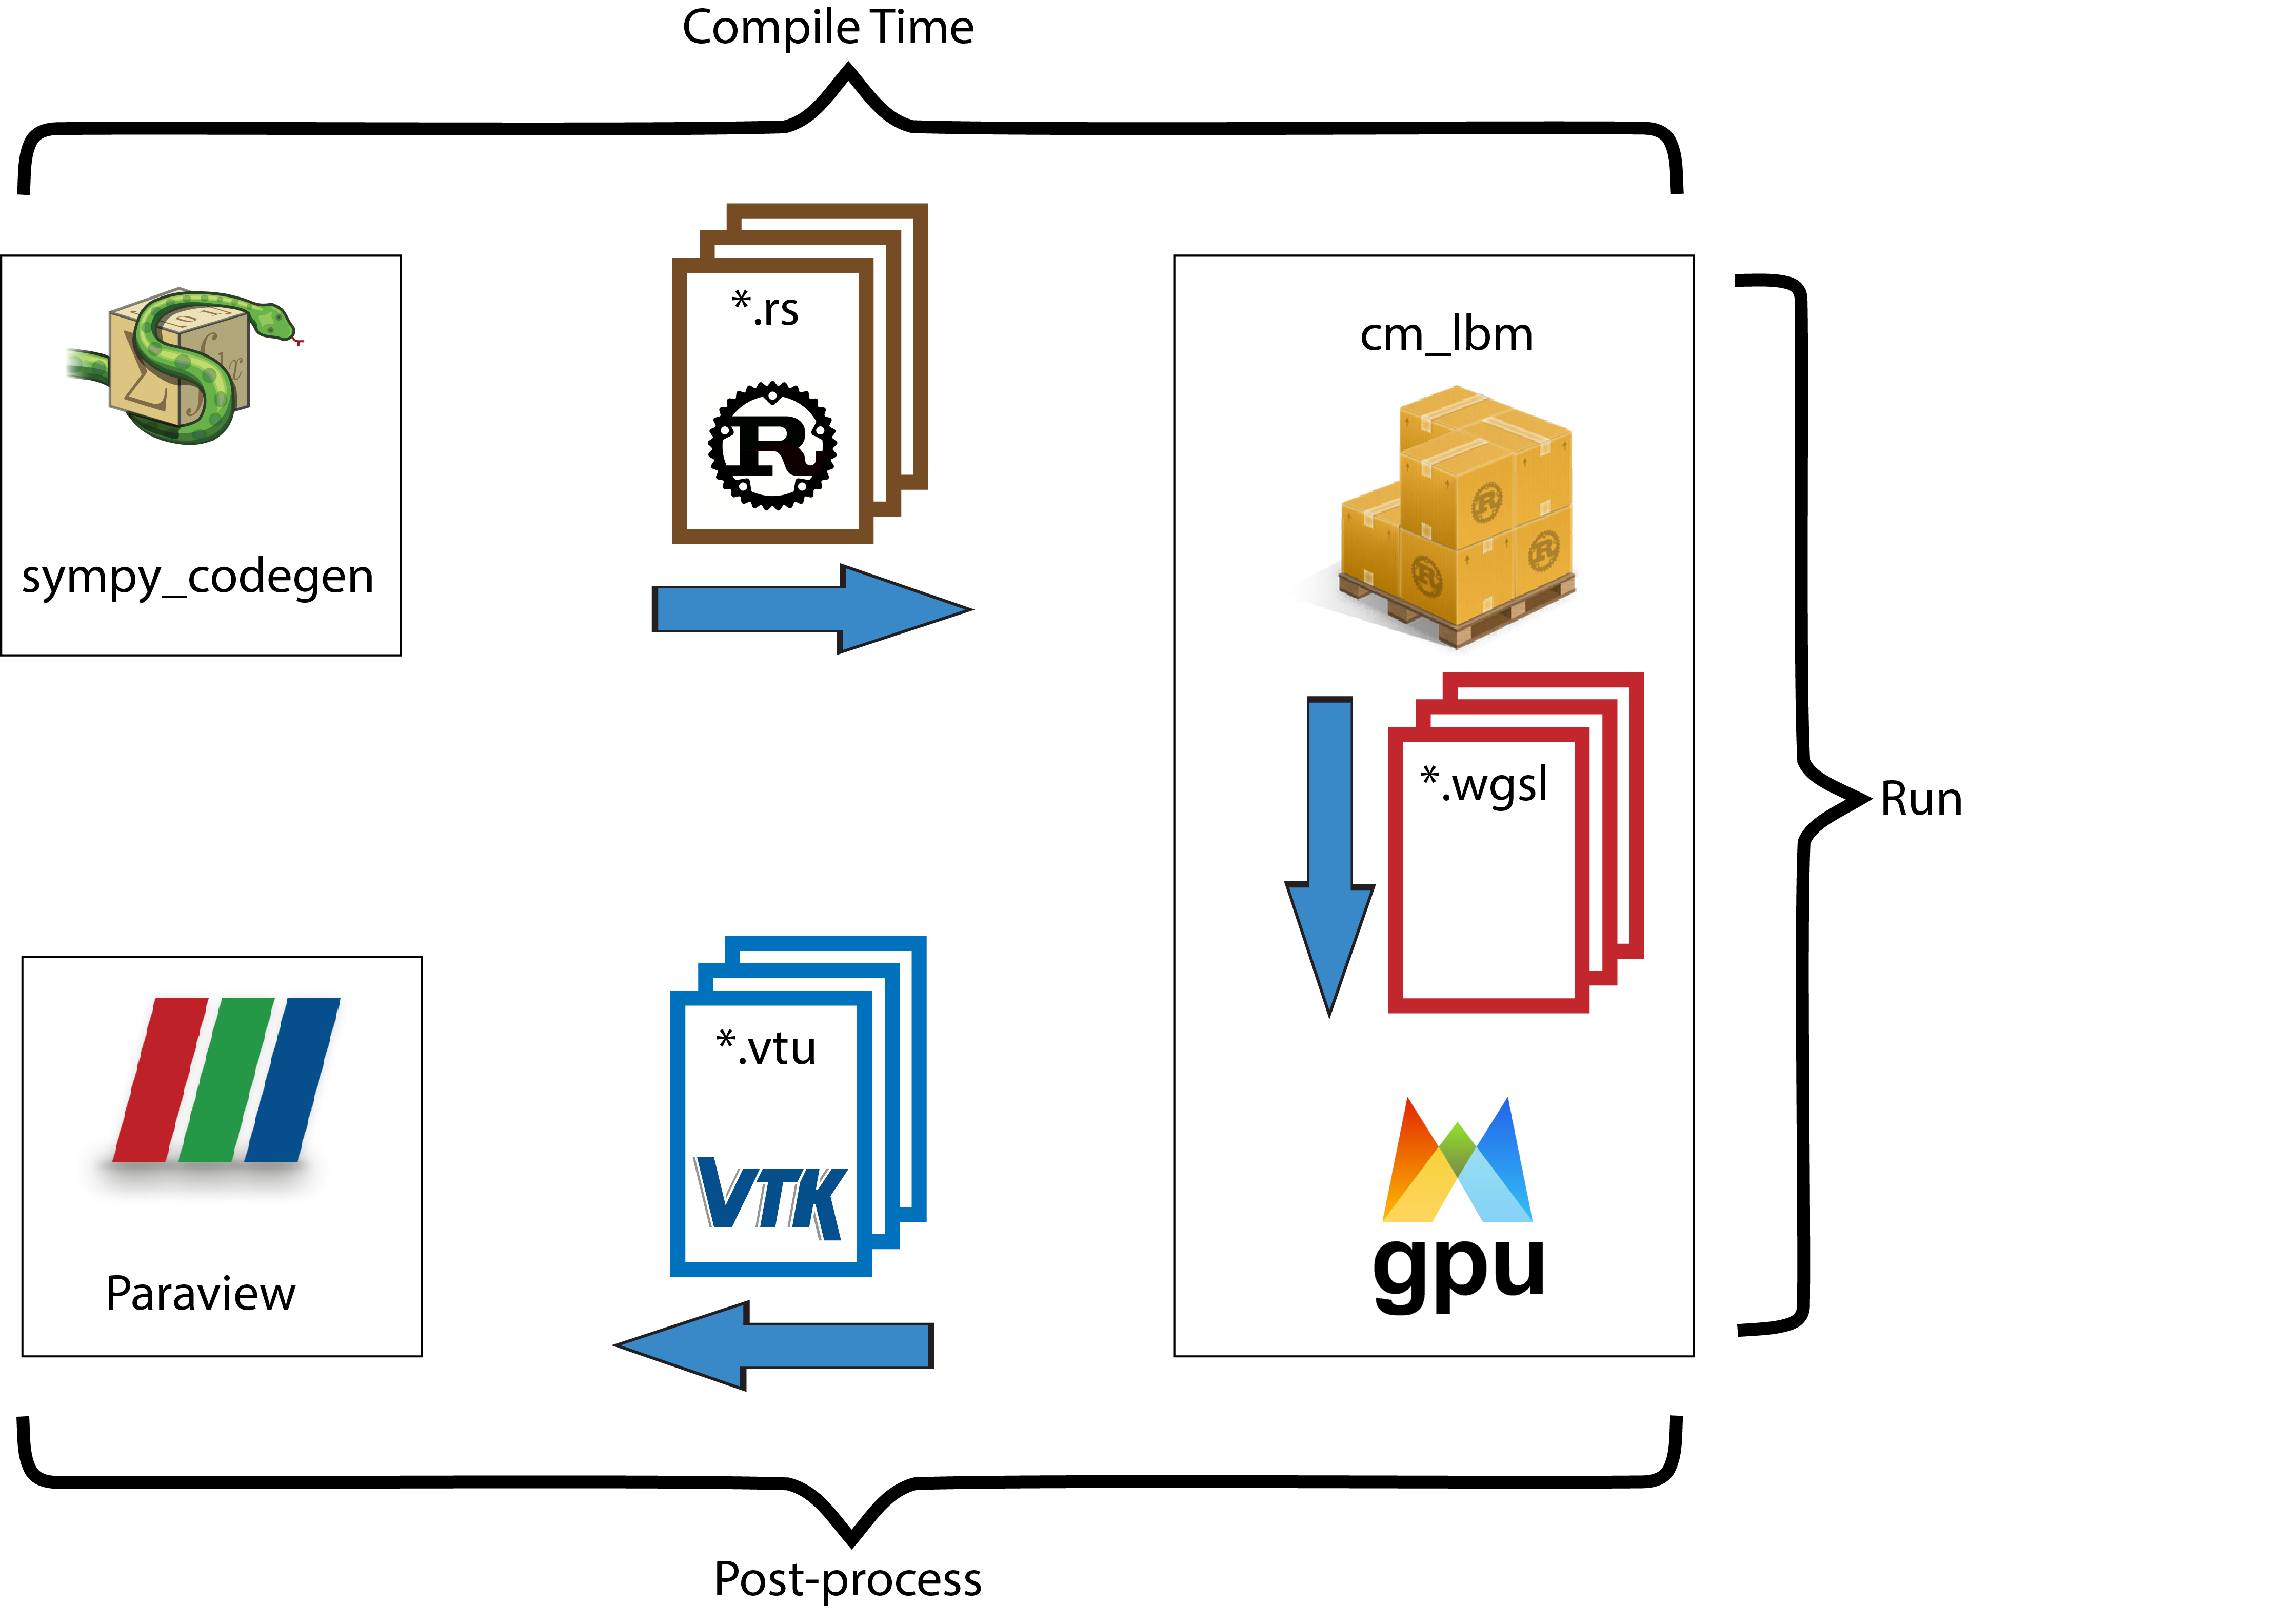
\includegraphics[width=\linewidth]{workflow.png}
\end{center}
  \caption{Generating a fluid dynamics image or movie
    has three phases. At compile time we use a
    python script uses SymPy to generate
  rust source files for the core LBM operators.
  At runtime, \lstinline{cm_lbm} generates WGSL shaders
  and uses them for compute pipelines.
  During the solve, VTK unstructured grid files are
  generated. 
  We post process those files into images using Paraview.
}
  \label{fig:architecture}
\end{figure}

\section{Implementation}\label{sec:implementation}
\subsection{Submission}
My submission zip contains pdf copies of this paper, my slides, and the original proposal. 
Also contained are
several mp4 videos, and a snapshot of the implementation source code.
\lstinline{README.md} in the source directory describes the contents
of the source directory,
though we will cover it at a high level in section \ref{sec:architecture}. 
The source code for the implementation can also be found on 
github\footnote{\url{https://github.com/SallySoul/lbm3}}
as well as the source code for two earlier 
prototypes\footnote{\url{https://github.com/SallySoul/wgpu_lbm_prototype}}\footnote{\url{https://github.com/SallySoul/lbm_clean}}.
The source for this paper and the slides can be found as 
part of another repository\footnote{\url{https://github.com/SallySoul/stencil_latex}} 
which is not included in the submission.

\subsection{Architecture}\label{sec:architecture}

Rendering my final movies required a pipeline of several tools,
but at the core is an LBM solver \lstinline{cm_lbm} written in Rust 
and running on an ARM Macbook.
See figure \ref{fig:architecture} for an overview.
LBM is detailed in section \ref{sec:relatedwork}. 
Working backwards, all of our renders
and figures were generated using 
Paraview\footnote{\url{https://www.paraview.org}}.
\lstinline{cm_lbm} generates 
VTK\footnote{\url{https://vtk.org}} files at set intervals as it 
steps through time during a solve.
The computational kernels used by the solver are 
compute shaders targeting WGPU\footnote{\url{https://wgpu.rs}},
see figure \ref{fig:compute_kernels} for an overview.
Several of these kernels are complex enough
to require a computer algebra system to generate.
To this end, a python script \lstinline{codegen.py}
is used to manipulate the equations from section \ref{sec:cm-mrt}
symbolically and generate
rust and wgsl implementations of the operations.
Strictly speaking, \lstinline{cm_lbm} is a library 
that bundles several example applications 
that hard code different simulations.

\subsection{Challenges}
The defining challenge while working on \lstinline{cm_lbm} was finding
the line between systems programming and high level abstractions.
On the systems side there were several notable issues.
Managing GPU resources requires a great deal of boiler plate.
Additionally, managing the various index spaces and translation
between them was an error prone part of development.
On the other hand, manipulating the LBM operators
demanded a high level representation that could be lowered
into WGSL.
I found it necessary to generate rust versions of these
operators as well for testing and debugging, as 
CPU based debugging is far simpler than doing so on the GPU.
SymPy expressions were the answer here as other projects have shown

Over the course of development, the trend was to move
more development into the higher level representation.
It is my belief that an ideal version of this implementation would
look more like a compiler than the current iteration.
I am certain that implementing any of the ideas from 
section \ref{sec:futurework}
would require more infrastructure be moved into the 
code generation phase.

Numerical Stability issues became an issue which
is evident in several of our renders.
Even now it is quite easy to feed in the wrong parameters
and quickly pollute the simulation with NaNs.
While utilizing double-precision numbers wasn't an option for me,
some possible avenues forward are described 
in section \ref{sec:futurework}

It goes without saying, 
but the timeline I proposed 
in no way correlates to the actual order of events.

\subsection{Tool Choice Reflection}
 wanted to use this project to access the suitability of Rust $+$ WGPU 
as a cross-platform compute target, 
while still taking advantage of platform specific features 
for this project.




I wanted to use this project to access the suitability of Rust $+$ WGPU 
as a cross-platform compute target.
M-GPUs can access far more RAM than is typically available to GPUs.
Given the memory intensive nature of LBM, this seemed advantageous.

I was happy using Rust to handle this project, as both the 
language and the surrounding ecosystem helped to manage
the complexity during development.
WGPU is a bit more nuanced: the cross-platform nature
is a tradeoff. In general WGPU, 
and the WebGPU standard it implements,
target the common denominator across most GPUs.
As a result, some desirable features and a more advanced
shading language are not available.
However, WGPU does expose the unified memory of M processors,
which is quite valuable.
CUDA would be a better choice 
for developing purpose built HPC
applications, but the freedom to utilize other GPU vendors is enticing.

Targeting my Macbook's GPU was a sensible choice for a course project.
While M1 GPUs don't support double precision, 
they are also a promising target for scientific computing \cite{Kenyon2022}.
I got favorable runtime results when compared to CPU based implementations,
and feel encouraged to continue exploring this avenue.

\begin{figure}
  \begin{center}
    \includegraphics[width=0.4\linewidth]{stream_0.png}
    \includegraphics[width=0.4\linewidth]{stream_1.png}

    \includegraphics[width=0.6\linewidth]{stream_2.png}
  \end{center}
  \caption{Stream example}
\end{figure}

\begin{figure}
  \begin{center}
    \includegraphics[width=\linewidth]{specular.png}
  \end{center}
  \caption{Specular Slip Boundaries.
For now we can add spheres, here we see those cells colored by the z component of the normal.}
\end{figure}
